\chapter{Electrochemistry}

\section{Pre-lesson exercise: Electrochemistry}
\subsection{Metals}
\subsubsection{Problem}
\bf{W}, \bf{X}, \bf{Y} and \bf{Z} are four unknown metals.

\bf{Y} does not react with water.

Precipitation is observed when solid \bf{W} is added into a solution of \bf{Z}
chloride.  No visible change is observed when solid \bf{W} is added into a solution
of \bf{Y} chloride.

Based on the above information, match the following metals to the correct
letters:
\begin{itemize}
	\item \ch{Mg}
	\item \ch{Al}
	\item \ch{Fe}
	\item \ch{Cu}
\end{itemize}

\subsubsection{Solution}

Since \bf{W} displaces \bf{Z} but not \bf{Y}, \bf{W} is more reactive than \bf{Z}
but less reactive than \bf{Y}. However, \bf{Y} does not react with water,
indicating that it is not highly reactive.

We can conclude that:
\begin{itemize}
	\item {\color{accent} \bf{W} is iron}. It has a reactivity in between that of two metals.
	\item {\color{accent} \bf{Z} is copper}. It has the lowest reactivity, since \bf{W} could displace it.
	\item {\color{accent} \bf{Y} is aluminium}. It is more reactive than \bf{W}, yet cannot dissolve in water, indicating that its reactivity is not the highest.
	\item {\color{accent} \bf{X} is, therefore, magnesium}.
\end{itemize}

\subsection{Electrolysis}
\subsubsection{Problem}
The electrolysis of dilute sodium nitrate was conducted as shown in Figure~\ref{fig:electrolysis-nano3}.
\begin{figure}[htpb]
	\centering
	\label{fig:electrolysis-nano3}
	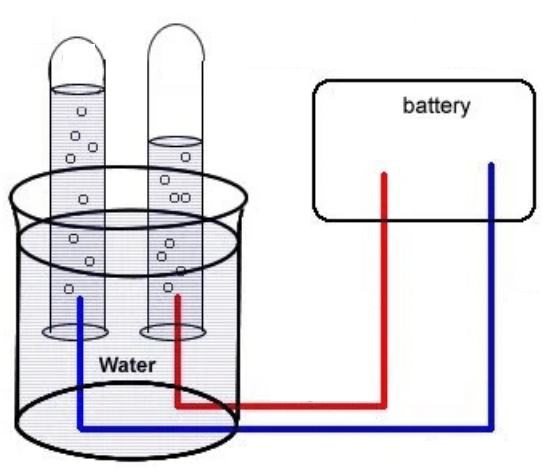
\includegraphics[width=0.4\linewidth]{assets/09_electrolysis_nano3.png}
	\caption{Electrolysis of \ch{NaNO3 \aq}}
\end{figure}

\begin{enumerate}
	\item With reference to oxidation numbers, explain why the nitrate anion will not be discharged. \label{part:no3-discharge}
	\item Explain why the sodium cation will not be discharged. \label{part:na-discharge}
	\item Despite Parts~\ref{part:no3-discharge} and~\ref{part:na-discharge}, explain why
	      the electrolysis will not work without sodium nitrate.
	\item By considering the oxidation and reduction reactions taking place, label the following on the diagram:
	      \begin{itemize}
		      \item the polarity of the battery (\(+\) or \(-\)),
		      \item the anode and the cathode, and
		      \item the flow of electrons, and the flow of electrical current.
	      \end{itemize}
	\item State what will be observed when a few drops of universal \pH\ indicator
	      are added into the solution.
\end{enumerate}

\subsubsection{Solution}
\ch{N} in \ch{NO3^-} has an oxidation state of \(+5\). Since \ch{N} is in
group 15 in the periodic table, \(+5\) is its maximum oxidation state. Since \ch{NO3^-}
is an anion, one would expect it to be oxidised at the anode. However, the
oxidation of \ch{NO3^-} is defined as the increase in oxidation state of \ch{N},
which is impossible. Therefore, \ch{NO3^-} cannot be oxidised.

The competing species at the cathode (to be reduced) are \ch{Na^+} and \ch{H2O}, since the electrolyte
is an aqueous solution. \ch{H2O}, however, is lower in the electrochemical series,
so it is preferentially reduced over \ch{Na^+}. The reduction of \ch{H2O}
forms \ch{H2 \gas{}}, and the reduction of \ch{Na^+} will only take place once
all \ch{H2O} has been reduced/oxidised.

Without \ch{NaNO3 \aq}, only \ch{H2O \lqd} would be present in the electrolyte.
Assuming that \ch{H2O \lqd} is deionised for the purposes of this electrolysis, it
will not allow electron flow without mobile ions which act as mobile charge carriers.

The annotated diagram is in Figure~\ref{fig:nano3-ans}.

\begin{figure}[htpb]
	\centering
	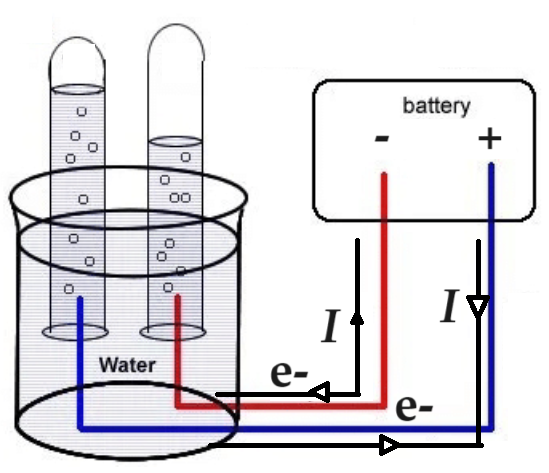
\includegraphics[width=0.4\linewidth]{assets/09_electrolysis_nano3_ans.png}
	\caption{Annotated electrolysis diagram}
	\label{fig:nano3-ans}
\end{figure}

\ch{H2O \lqd} is both preferentially reduced and oxidised at the cathode and anode
respectively.
\begin{align*}
	\ch{2 H2O \lqd{} + 2 e- & <=> H2 \gas{} + 2 OH^- \aq}             \\
	\ch{H2O \lqd{}          & <=> 1/2 O2 \gas{} + 2 H^+ \aq{} + 2 e-}
\end{align*}
For the same number of moles of electrons passed through the electrolyte, the
number of moles of \ch{OH^-} and \ch{H^+} produced are equal. The overall \pH\
of the solution does not change.

However, \ch{H^+} ions are produced at the anode, meaning that the solution surrounding
the anode will turn {\color{accent} acidic}. {\color{accent} Near the anode, the green universal
\pH\ indicator will turn red}.

\ch{OH^-} ions are produced at the cathode, meaning that the solution surrounding
the cathode will turn {\color{cobalt} basic}. {\color{cobalt} Near the cathode, the green universal \pH\ indicator will turn purple.}

% *** *** ***
\section{Homework: Electrochemistry}

\subsection{Electrochemical cells}
\subsubsection{Problem}
A \bf{standard} electrochemical cell is prepared involving two reactions: the
oxidation of sodium sulfate into sodium peroxydisulfate (\ch{Na2S2O8}) and the
reduction of iron(III) chloride into iron(II) chloride. Write down the cell
reaction for the above cell.

Given the following \(E^\standardstate\) values, determine if the following
statements are true or false.

\begin{align*}
	\ch{S2O8^{2-} \aq{} + 2 e- <=> 2 SO4^{2-} \aq} & \quad E^\standardstate = +\qty{2.05}{\volt} \\
	\ch{Fe^{3+} \aq{} + e- <=> Fe^{2+} \aq}        & \quad E^\standardstate = +\qty{0.77}{\volt}
\end{align*}

\begin{enumerate}
	\item The equilibrium constant of the cell reaction is very small.
	\item If the platinum foils are connected directly, the colour of the \ch{"\ox{2,Fe}"}/\ch{"\ox{3,Fe}"} solution
	      intensifies.
	\item When connected in the conventional way, this cell cannot light up an LED bulb.
	\item If we mix aqueous iron(III) sulfate with potassium persulfate (\ch{K2S2O8}), the solution will
	      turn from yellow to pale green.
	\item Swapping the two half-cells around generates a battery of voltage \qty{1.28}{\volt}.
\end{enumerate}

\subsubsection{Solution}
The cell reaction \sidenote{A combination of the two half-reactions.} is
\begin{equation*}
	\ch{2 SO4^{2-} \aq{} + 2 Fe^{3+} \aq{} -> S2O8^{2-} \aq{} + 2 Fe^{2+} \aq}
\end{equation*}

If a reaction has a small equilibrium constant, the equilibrium position favours
the reactants. The products do not form spontaneously. At the same time,
\begin{align*}
	E^\standardstate_\text{cell} & = E^\standardstate_\text{cathode} - E^\standardstate_\text{anode} \\
	                             & = 0.77 - 2.05                                                     \\
	                             & = \qty{-1.28}{\volt}                                              \\
	                             & < 0
\end{align*}
\(E^\standardstate_\text{cell} < 0\) confirms that the reaction is not spontaneous.
Therefore, it is {\color{accent} true} that the reaction has a small equilibrium
constant.

If the platinum electrodes are connected directly, the circuit will be shorted.
Since \(E_\text{cell} = E^\standardstate_\text{cell} < 0\), electrons will flow
in the opposite direction and the reverse of the cell reaction occurs. \ch{Fe^{3+} \aq}
will be formed from \ch{Fe^{2+} \aq}, so it is {\color{accent} true} that the colour of the solution
intensifies to a deeper yellow-orange as \ch{[Fe^{3+}]} increases.

Since \(E_\text{cell} < 0\), electrons cannot flow in the cell when connected
conventionally. Therefore, it is {\color{accent} true} that an LED bulb cannot
light up.

Since the equilibrium position favours the reaction's reactants and not its
products, the increased concentration of \ch{S2O8^{2-} \aq} will hinder
the rate of reaction of \ch{SO4^{2-} \aq} and \ch{Fe^{3+} \aq} further.
It is unlikely that a large amount of \ch{Fe^{3+} \aq} will be used up, and
therefore {\color{accent} untrue} that the yellow colour of \ch{Fe^{3+} \aq}
will turn into the pale-green colour of \ch{Fe^{2+} \aq}.

Swapping the two electrodes causes the reverse reaction to occur. The reverse
reaction occurs more readily and electrons will flow in the opposite direction,
producing a battery whose voltage is the negative of the cell potential, i.e.
\qty{1.28}{\volt}.

\subsection{Spontaneous reactions}
\subsubsection{Problem}
A list of values (in alphabetical order) is provided below. Use the relevant values to
determine if a reaction is spontaneous and write a balanced equation for those reactions
which are spontaneous.

\begin{alignat*}{3}
	\ch{Ag+ \aq{} + \el{}                   & <=> Ag \sld} \quad                  & E^\standardstate & = +\qty{0.80}{\volt} \\
	\ch{Cl2 \gas{} + 2 \el{}                & <=> 2 Cl- \aq} \quad                & E^\standardstate & = +\qty{1.36}{\volt} \\
	\ch{ClO2^- \aq{} + H2O \lqd{} + 2 \el{} & <=> ClO- \aq{} + 2 OH- \aq} \quad   & E^\standardstate & = +\qty{0.59}{\volt} \\
	\ch{Fe^2+ \aq{} + 2 \el{}               & <=> Fe \sld} \quad                  & E^\standardstate & = \qty{-0.44}{\volt} \\
	\ch{Fe^3+ \aq{} + 3 \el{}               & <=> Fe \sld} \quad                  & E^\standardstate & = \qty{-0.04}{\volt} \\
	\ch{Fe^3+ \aq{} + \el{}                 & <=> Fe^2+ \aq} \quad                & E^\standardstate & = +\qty{0.77}{\volt} \\
	\ch{Fe(OH)3 \sld{} + \el{}              & <=> Fe(OH)2 \sld{} + OH- \aq} \quad & E^\standardstate & = \qty{-0.56}{\volt} \\
	\ch{I2 \sld{} + 2 \el{}                 & <=> 2 I- \aq} \quad                 & E^\standardstate & = +\qty{0.54}{\volt} \\
	\ch{Na+ \aq{} + \el{}                   & <=> Na \sld} \quad                  & E^\standardstate & = \qty{-2.71}{\volt} \\
	\ch{NO3^- \aq{} + 2 H+ \aq{} + \el{}    & <=> NO2 \gas{} + H2O \lqd} \quad    & E^\standardstate & = +\qty{0.81}{\volt} \\
	\ch{SO4^2- \aq{} + 4 H+ \aq{} + 2 \el{} & <=> SO2 \gas{} + 2 H2O \lqd} \quad  & E^\standardstate & = +\qty{0.17}{\volt} \\
\end{alignat*}

\begin{enumerate}
	\item Mixing aqueous iron(III) sulfate with acidified aqueous iron(II) sulfate
	\item Bubbling chlorine gas through alkaline aqueous sodium chlorate(I)
	\item Reducing iron(III) hydroxide with aqueous potassium iodide
	\item Dropping an iron nail into aqueous iron(III) chloride
	\item Dropping silver into concentrated nitric acid
\end{enumerate}

\subsubsection{Mixing aqueous iron(III) sulfate with acidified aqueous iron(II) sulfate}
The cell reaction is
\begin{equation*}
	\ch{Fe^3+ \aq{} + Fe^2+ \aq{} -> Fe^2+ \aq{} + Fe^3+ \aq}
\end{equation*}
where \ch{Fe^3+ \aq} had been reduced and \ch{Fe^2+ \aq} had been oxidised.
Therefore,
\begin{align*}
	E^\standardstate_\text{cell} & = +0.77 - (+0.77)   \\
	                             & = \qty{0.00}{\volt}
\end{align*}
The reaction mixture is {\color{accent} in equilibrium} under standard conditions.

\subsubsection {Bubbling chlorine gas through alkaline aqueous sodium chlorate(I)}
The cell reaction is
\begin{equation*}
	\ch{ClO- \aq{} + Cl2 \gas{} + 2 OH- \aq{} -> ClO2^- \aq{} + 2 Cl- \aq{} + H2O \lqd{} + 2 \el}
\end{equation*}
and
\begin{align*}
	E^\standardstate_\text{cell} & = +1.36 - (-0.59)       \\
	                             & = \qty{1.95}{\volt} > 0
\end{align*}
The reaction is {\color{accent} spontaneous}.

\subsubsection {Reducing iron(III) hydroxide with aqueous potassium iodide}
The cell reaction is
\begin{equation*}
	\ch{2 Fe(OH)3 \sld{} + 2 I- \aq{} -> 2 Fe(OH)2 \sld{} + I2 \lqd{} + 2 OH- \aq}
\end{equation*}
and
\begin{align*}
	E^\standardstate_\text{cell} & = -0.56 - (-0.54)        \\
	                             & = \qty{-0.02}{\volt} < 0
\end{align*}
The reaction is {\color{accent} not spontaneous}, but its reverse is under
standard conditions.

\subsubsection{Dropping an iron nail into aqueous iron(III) chloride}
The cell reaction is \sidenote{This is a synproportionation!}
\begin{equation*}
	\ch{Fe \sld{} + 2 Fe^3+ \aq{} -> 3 Fe^2+ \aq}
\end{equation*}
and
\begin{align*}
	E^\standardstate_\text{cell} & = +0.77 - \ab(+0.44)     \\
	                             & = +\qty{0.33}{\volt} > 0
\end{align*}
The reaction here is {\color{accent} spontaneous}.

\subsubsection{Dropping silver into concentrated nitric acid}

The cell reaction is
\begin{equation*}
	\ch{Ag \sld{} + NO3^- \aq{} + 2 H+ \aq{} ->  Ag+ \aq{} + NO2 \gas{} + H2O \lqd}
\end{equation*}
and
\begin{align*}
	E^\standardstate_\text{cell} & = +0.81 - \ab(-0.80)     \\
	                             & = +\qty{1.61}{\volt} > 0
\end{align*}
The reaction here is {\color{accent} spontaneous}.

\subsection{Calculations}
\subsubsection{Problem}
\begin{enumerate}
	\item Calculate the time needed for a constant current of \qty{1.20}{\ampere} to produce
	      \qty{0.500}{\gram} of elemental thallium on a cathode, from a solution of \ch{"\ox{1,Tl}"}
	      ions.

	\item Under suitable conditions, we can deposit the oxide \ch{Co3O4} on an anode
	      from the electrolysis of a \ch{"\ox{2,Co}"} source. Calculate the minimum current
	      required to deposit \qty{2.00}{\gram} of the oxide on the anode within \qty{1}{\hour}.

	\item \qty{.2416}{\gram} of a water-insoluble, monoprotic carboxylic acid was measured out
	      and mixed with a concentrated sodium chloride solution with constant stirring. After
	      electrolysing the concentrated solution for \qty{5.40}{\minute} with a constant current
	      of \qty{367}{\milli\ampere}, all the organic acid dissolved. Determine the molar mass
	      of the acid and suggest a possible structure.
\end{enumerate}

\subsubsection{Solution: Thallium deposition}
We can write the reduction of \ch{"\ox{1,Tl}"} as
\begin{equation*}
	\ch{Tl+ \aq{} + \el{} -> Tl \sld}
\end{equation*}
where one mole of electrons is required for one mole of solid thallium to be deposited.
\begin{align*}
	\eta_{ \el{} } = \eta_{ \ch{Tl+} } & = \f{ \qty{0.500}{\gram} }{ \qty{204.4}{\gram\per\mol} }                                     \\
	                                   & = \qty{2.446e-3}{\mol}                                                                       \\
	\\
	n_{ \el{} }                        & = \ab( \qty{2.446e-3}{\mol} ) \times \ab( \qty{6.02e23}{\per\mol} )                          \\
	                                   & = \num{1.473e21}                                                                             \\
	\\
	\because\; Q = It                  & = ne                                                                                         \\
	\therefore\; t                     & = \f{ne}{I}                                                                                  \\
	                                   & = \f{ \ab( \num{1.473e21} ) \times \ab( \qty{1.602e-19}{\coulomb} ) }{ \qty{1.20}{\ampere} } \\
	                                   & = \color{accent} \qty{196.6}{\second}
\end{align*}

\subsubsection{Solution: Cobalt oxide??}
\begin{align*}
	\eta_{ \ch{Co3O4} } & = \f{ \num{2.00} }{ 58.9 \times 3 + 16.0 \times 4 } \\
	                    & = \qty{ 8.309e-3 }{ \mol }                          \\
\end{align*}
We can write the oxidation of \ch{"\ox{2,Co}"} into \ch{Co3O4} as
\begin{equation*}
	\ch{3 Co^2+ \aq{} + 4 H2O \lqd{} -> Co3O4 \sld{} + 8 H+ \aq{} + 2 \el{}}
\end{equation*}
For every mole of \ch{Co3O4} deposited, \qty{2}{\mol} of electrons are passed.
\begin{align*}
	\eta_{ \el{} } & = \ab(\qty{8.309e-3}{\mol}) \times 2                                          \\
	n_{ \el{} }    & = \ab[\ab(\qty{8.309e-3}{\mol}) \times 2] \times \ab(\qty{6.02e23}{\per\mol}) \\
	               & = \num{1.000e22}
\end{align*}
We can do something similar to what we've done previously.
\begin{align*}
	\because \; Q = It & = ne                                                                                                        \\
	\therefore \; I    & = \f{ne}{t}                                                                                                 \\
	                   & = \f{ \ab(\num{1.000e22}) \times \ab( \qty{1.602e-19}{\coulomb} ) }{ 1 \times 60 \times \qty{60}{\second} } \\
	                   & = \color{accent} \qty{4.45}{\deci\ampere}
\end{align*}

\subsubsection{Solution: Organic chemistry (again)}
We have to work backwards. Let's start by finding the amount of electrons passed.
\begin{align*}
	\because \; Q = I t & = n e                                                                                                                                   \\
	\therefore \; n     & = \f{I t}{e}                                                                                                                            \\
	                    & = \f{ \ab( \qty{367e-3}{\ampere} ) \times \ab( \qty{5.40}{\minute} \times \qty{60}{\second\per\minute} ) }{ \qty{1.602e-19}{\coulomb} } \\
	                    & = \num{7.422e20}                                                                                                                        \\
	\eta_{ \el{} }      & = \f{ \num{7.422e20} }{ \qty{6.02e23}{\per\mol} }                                                                                       \\
	                    & = \qty{1.233e-3}{\mol}
\end{align*}
The electrolysis of concentrated sodium chloride solution (or brine) can be written as
\begin{align*}
	\ch{2 H2O \lqd{} + 2 \el{} & -> H2 \gas{} + 2 OH- \aq} \\
	\ch{2 Cl- \aq{}            & -> Cl2 \gas{} + 2 \el}    \\
\end{align*}
For every \qty{2}{\mol} of \ch{OH- \aq} produced, \qty{2}{\mol} of electrons
were passed. The \ch{OH- \aq} were crucial in neutralising the carboxylic acid.
\begin{align*}
	\eta_{ \ch{OH-} } & = \eta_{ \el{} }       \\
	                  & = \qty{1.233e-3}{\mol}
\end{align*}
Let the carboxylic acid be \ch{R-COOH}. Since the acid had been completely
neutralised, \( \eta_{ \ch{H+} } = \eta_{ \ch{OH-} } \).
\begin{align*}
	\eta_{ \ch{R-COOH} }   & = \eta_{ \ch{OH-} }                                       \\
	                       & = \qty{1.233e-3}{\mol}                                    \\
	M_r                    & = \f{ \qty{.2416}{\gram} }{ \qty{1.233e-3}{\mol} }        \\
	                       & = \color{accent} \qty{195.95}{\gram\per\mol}              \\
	M_r \text{ of \ch{R} } & = \qty{195.95}{\gram\per\mol} - \qty{45.0}{\gram\per\mol} \\
	                       & = \qty{150.95}{\gram\per\mol}
\end{align*}
